% !TeX root = main.tex
\documentclass[11pt,a4paper]{article}
% Tata letak bersama. Konten setiap bagian berada di sections/ dan appendices/.
\usepackage[T1]{fontenc}
\usepackage{lmodern}
\usepackage[bahasa]{babel}
\usepackage[margin=25mm,headheight=15pt]{geometry}
\usepackage{microtype}
\usepackage{graphicx,booktabs,tabularx,longtable,array}
\usepackage[table]{xcolor}
\usepackage{amsmath,enumitem,float,fancyhdr,titlesec,listings}
\usepackage{xurl}
\usepackage{pdflscape}
\usepackage[section]{placeins}
\usepackage{needspace,etoolbox}
\pretocmd{\section}{\Needspace{6\baselineskip}}{}{}
\definecolor{Navy}{HTML}{17324D}
\definecolor{Teal}{HTML}{087F8C}
\definecolor{Pale}{HTML}{F0F5F8}
\definecolor{Muted}{HTML}{566573}
\usepackage[colorlinks=true,linkcolor=Navy,urlcolor=Teal,citecolor=Teal,bookmarksnumbered=true]{hyperref}
\hypersetup{pdftitle={IF4031 M1 - AkuAnakTehat},pdfauthor={Dzaky Aurelia Fawwaz; Muhammad Alfansya}}
\setlength{\parindent}{0pt}
\setlength{\parskip}{5pt}
\setlength{\emergencystretch}{3em}
\renewcommand{\arraystretch}{1.18}
\setlist{itemsep=2pt,topsep=4pt,leftmargin=*}
\newcolumntype{Y}{>{\raggedright\arraybackslash}X}
\newcolumntype{P}[1]{>{\raggedright\arraybackslash}p{#1}}
\titleformat{\section}{\Large\bfseries\color{Navy}}{\thesection}{0.7em}{}
\titleformat{\subsection}{\large\bfseries\color{Navy}}{\thesubsection}{0.7em}{}
\titleformat{\subsubsection}{\normalsize\bfseries\color{Teal}}{\thesubsubsection}{0.7em}{}
\pagestyle{fancy}
\fancyhf{}
\fancyhead[L]{\small IF4031: Milestone 1}
\fancyhead[R]{\small AkuAnakTehat}
\fancyfoot[L]{\scriptsize Platform Koordinasi Kebencanaan BNPB}
\fancyfoot[R]{\thepage}
\renewcommand{\headrulewidth}{0.3pt}
\raggedbottom
\lstdefinelanguage{Golang}{morekeywords={func,return,if,else,for,range,var,const,type,struct,map,select,case,default,go,defer,package,import,nil,true,false,continue},sensitive=true,morecomment=[l]{//},morestring=[b]"}
\lstset{basicstyle=\fontsize{8}{10}\selectfont\ttfamily,keywordstyle=\color{Navy}\bfseries,commentstyle=\color{Muted},stringstyle=\color{Teal},breaklines=true,breakatwhitespace=false,columns=fullflexible,keepspaces=true,showstringspaces=false,frame=single,rulecolor=\color{Navy!25},backgroundcolor=\color{Pale},numbers=left,numberstyle=\tiny\color{Muted},numbersep=6pt,xleftmargin=10pt,framexleftmargin=3pt,captionpos=b,tabsize=2}
\newcommand{\codepath}[1]{\href{\RepoURL/blob/\CodeRevision/#1}{\nolinkurl{#1}}}
\newcommand{\evidence}[1]{\codepath{docs/evidence/integration/#1}}
\newcommand{\pending}[1]{\par\smallskip\noindent\fcolorbox{orange!60!black}{orange!7}{\parbox{0.93\linewidth}{\raggedright\textbf{Perlu dilengkapi:} #1}}\par\smallskip}
\newcommand{\diagram}[3]{\begin{figure}[htbp]\centering\includegraphics[width=\linewidth,height=0.76\textheight,keepaspectratio]{assets/figures/#1.pdf}\caption{#2}\label{#3}\end{figure}}
\newcommand{\architecturefigure}{\clearpage\begin{landscape}\begin{figure}[p]\centering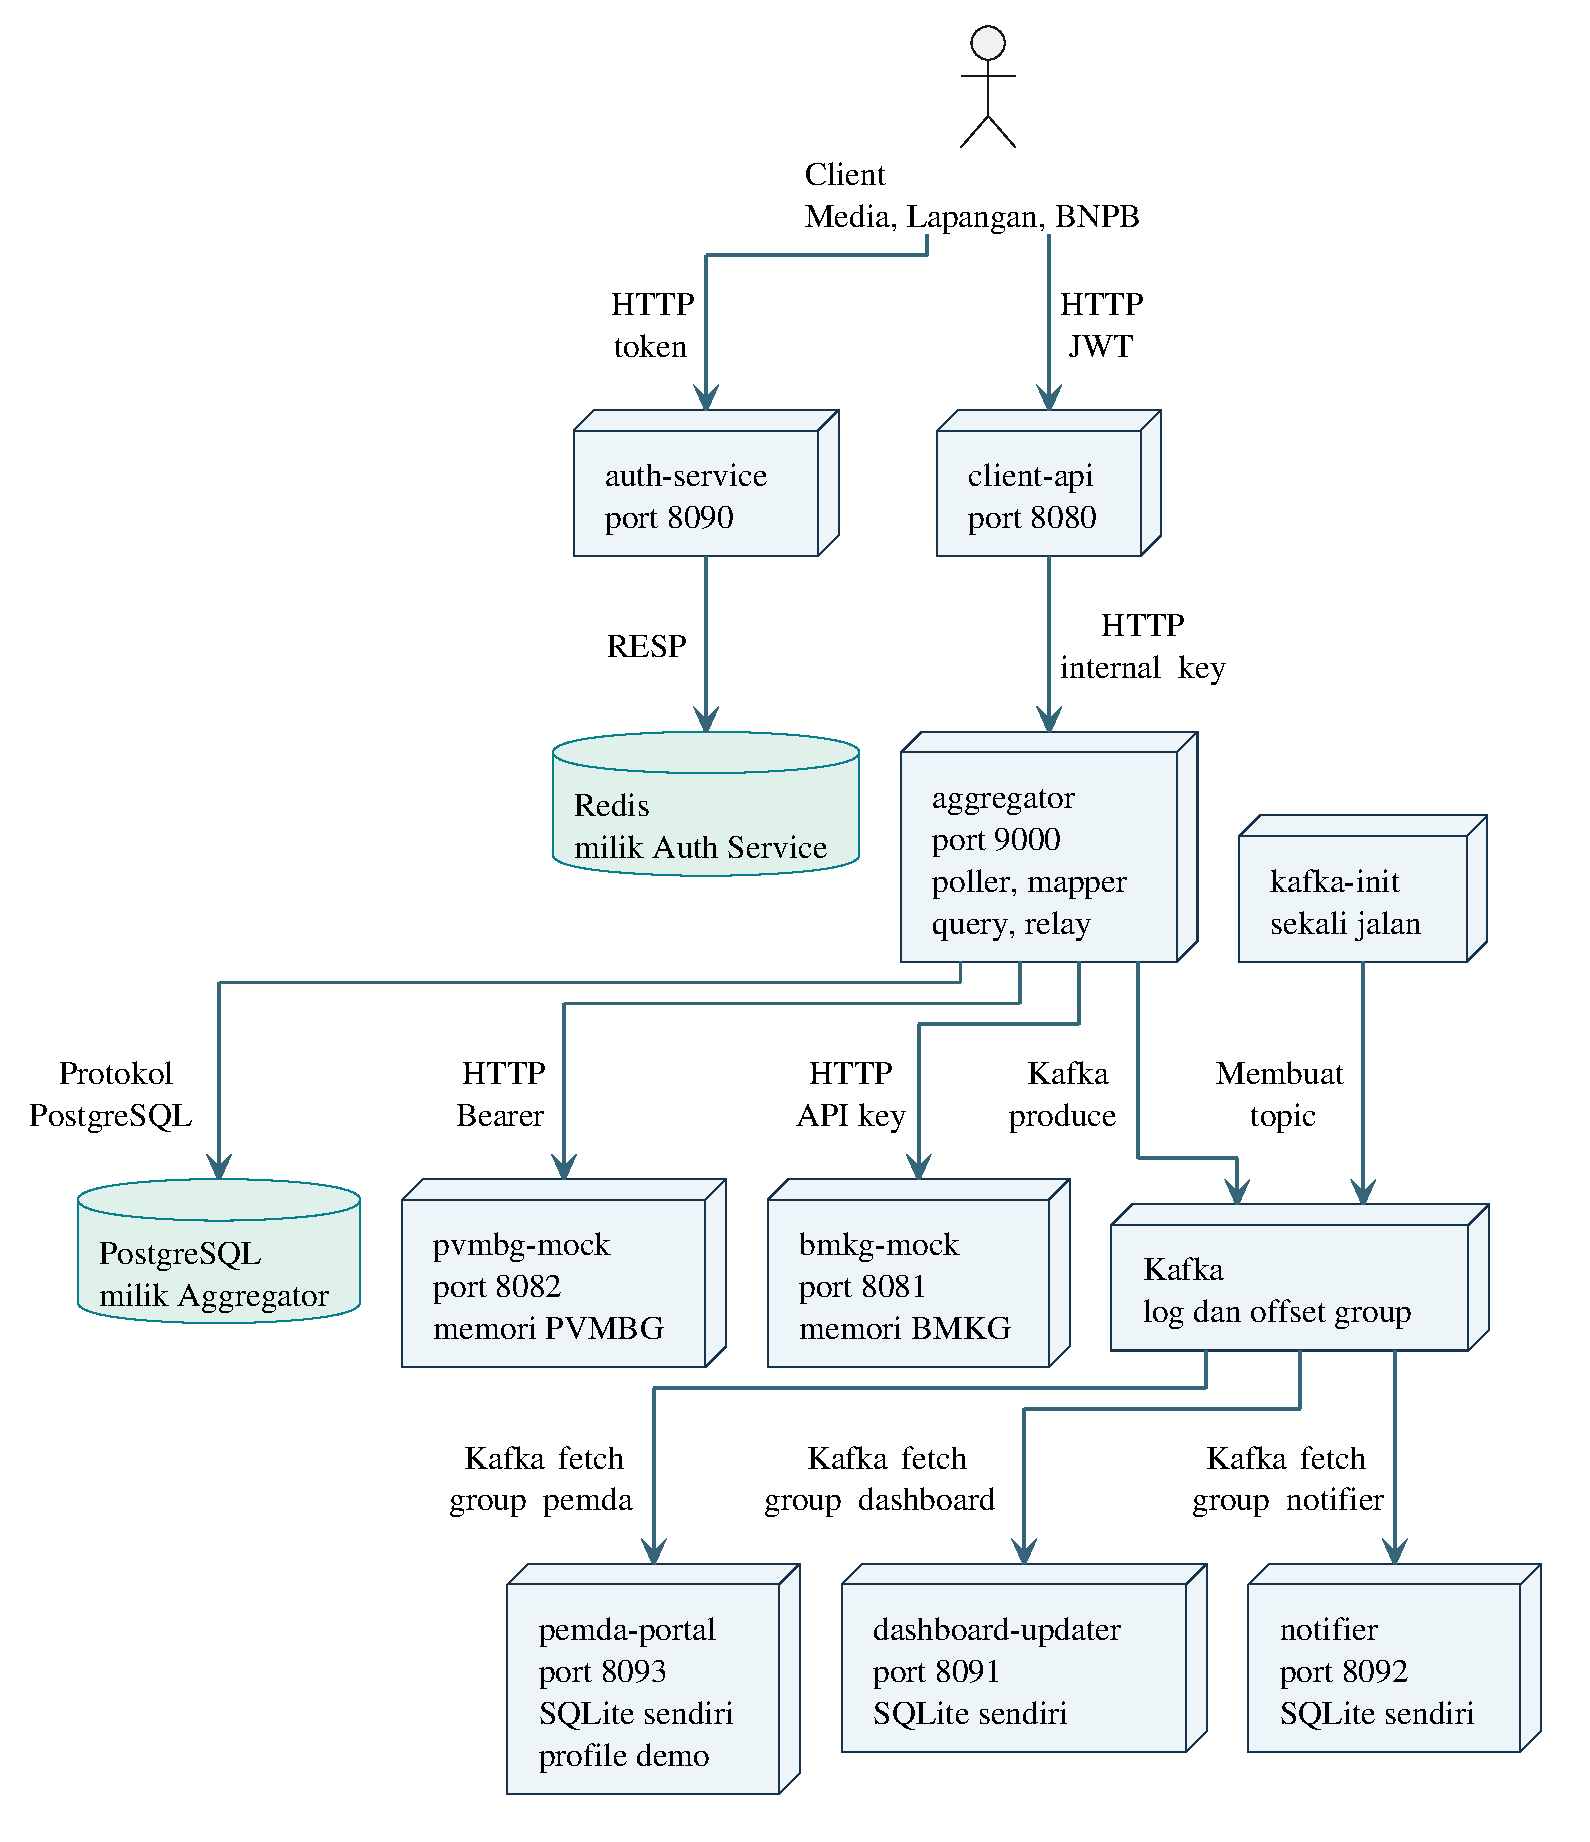
\includegraphics[width=\linewidth,height=0.84\textwidth,keepaspectratio]{assets/figures/01-arsitektur.pdf}\caption{Service, protokol, storage ownership, dan batas container. Memori mock dan SQLite berada pada container pemilik. Panah Kafka ke consumer menunjukkan aliran data; consumer menginisiasi fetch.}\label{fig:architecture}\end{figure}\end{landscape}}
\newcommand{\coderef}[1]{\par{\footnotesize\textbf{Acuan implementasi:} \codepath{#1}.}\par}
\newcommand{\proof}[1]{\par{\footnotesize\textbf{Bukti eksekusi:} \evidence{#1}.}\par}

% Ubah identitas dan tanggal di sini; jangan mengganti tanggal bukti pengujian.
\newcommand{\GroupName}{AkuAnakTehat}
\newcommand{\SystemName}{Platform Koordinasi Kebencanaan BNPB}
\newcommand{\ReportDate}{8 Oktober 2026}
\newcommand{\EvidenceDate}{6 Oktober 2026}
\newcommand{\RepoURL}{https://github.com/WwzFwz/AkuAnakTehat}
\newcommand{\CodeRevision}{f6e99cc10fec64042eb184c9d7f92d14cb22fd23}
\newcommand{\DemoEvidenceRevision}{811e3144c2b94021e0fba483a3a194a3d665af32}
\newcommand{\DzakyWriting}{\textit{[Isi kontribusi penulisan Dzaky]}}
\newcommand{\AlfanWriting}{\textit{[Isi kontribusi penulisan Muhammad Alfansya]}}

\begin{document}
\special{pdf:minorversion 7}
\hypersetup{pageanchor=false}
% !TeX root = ../main.tex
\begin{titlepage}
\centering
\vspace*{12mm}
{\color{Teal}\large LAPORAN TUGAS BESAR}\par
\vspace{5mm}
{\color{Navy}\Huge\bfseries Sistem Terdistribusi Dasar}\par
\vspace{5mm}
{\Large Milestone 1}\par
\vspace{10mm}
{\LARGE\bfseries\SystemName}\par
\vspace{4mm}
\rule{0.75\linewidth}{0.5pt}\par
\vspace{12mm}
{\Large Kelompok \textbf{\GroupName}}\par
\vspace{8mm}
\begin{tabular}{ll}
Dzaky Aurelia Fawwaz & 13523065\\[3mm]
Muhammad Alfansya & 13523005
\end{tabular}
\vfill
{\large IF4031 Arsitektur Aplikasi Terdistribusi}\par
\vspace{3mm}
{\ReportDate}\par
\vspace{8mm}
{\small Sumber LaTeX dan diagram disertakan dalam repository.\\
Revisi implementasi acuan \texttt{f6e99cc}.\\
Bukti pengujian lokal bertanggal \EvidenceDate.}
\end{titlepage}

\pagenumbering{roman}
\hypersetup{pageanchor=true}
% !TeX root = ../main.tex
\section*{Kontribusi Anggota}
\addcontentsline{toc}{section}{Kontribusi Anggota}
Pembagian berikut menjelaskan kontribusi setiap anggota berdasarkan komponen sistem dan tanggung jawab yang dikerjakan.

\begin{tabularx}{\linewidth}{P{0.22\linewidth}YY}
\toprule
Aspek & Dzaky Aurelia Fawwaz (13523065) & Muhammad Alfansya (13523005)\\
\midrule
Perancangan & Perancangan arsitektur sistem dan mekanisme penyelesaian P1 hingga P5. & Membantu verifikasi dan validasi kesesuaian rancangan terhadap spesifikasi.\\
Implementasi & BMKG Mock dan PVMBG Mock; Auth Service; polling, pemetaan, korelasi tsunami, transaksi dan watermark pada Aggregator; outbox relay dan producer Kafka; Dashboard Updater, Notifier, dan Pemda Portal; infrastruktur Docker Compose, bootstrap secret, dan CI; integrasi serta pengujian lintas komponen. & Query dan API internal Aggregator; Client API beserta rate limit, batas konkurensi, pagination, dan penanganan galat; CLI Tim Lapangan; serta script load test k6.\\
Penulisan laporan & \DzakyWriting & \AlfanWriting\\
\bottomrule
\end{tabularx}

\pending{Konfirmasi dan isi kontribusi penulisan kedua anggota pada \nolinkurl{metadata.tex} sebelum pengumpulan. Tidak ada persentase kontribusi yang diasumsikan.}

Laporan disusun dari kode yang telah diintegrasikan, bukti eksekusi lokal, dan rancangan awal kelompok. Bantuan LLM dijelaskan secara eksplisit pada Bagian~\ref{sec:ai}; tanggung jawab pemahaman dan verifikasi akhir berada pada kelompok.
\clearpage

\tableofcontents
\clearpage
\pagenumbering{arabic}
% !TeX root = ../main.tex
\section{Deskripsi Umum dan Lingkup}
BNPB membutuhkan representasi yang konsisten atas informasi gempa, potensi tsunami, dan aktivitas gunung api dari dua instansi yang otonom. BMKG dan PVMBG memiliki skema, kredensial, serta karakteristik latensi berbeda. Sistem ini mengambil data melalui polling, memetakannya menjadi \texttt{HazardEvent}, menyajikan data sesuai hak akses client, dan menyalurkan perubahan melalui broker kepada consumer independen.

Lingkup Milestone 1 mengikuti dokumen spesifikasi M1 dan konteks tugas terpusat~\cite{spec-m1,spec-central}. Kedua instansi berupa mock yang dibangun kelompok; data serta referensi gunung api bersifat sintetis. Tiga identitas downstream adalah Media, Tim Lapangan, dan BNPB Pusat. Seluruh akses downstream bersifat baca saja. Pelaporan dari lapangan, integrasi sistem instansi nyata, dan pengoperasian banyak instance tidak termasuk implementasi ini.

\subsection{Prinsip rancangan}
Tiga alur utama dipisahkan. Jalur ingest menangani ketidakpastian sumber; jalur baca menggunakan data yang sudah tersimpan; jalur event memindahkan perubahan melalui outbox dan Kafka. Pemisahan ini membuat satu request client tidak harus menunggu HTTP ke instansi sumber. Sebagai konsekuensi, hasil baca bukan data real-time langsung dari sensor: kebaruan harus dijelaskan melalui waktu data dan status sumber.

\begin{tabularx}{\linewidth}{lY}
\toprule Problem & Mekanisme inti yang diimplementasikan\\\midrule
P1 & Tolerant reader JSON, pemetaan kanonik, korelasi warning, dan preservasi field tambahan.\\
P2 & Worker per sumber, baca dari store, timeout, circuit breaker, batas konkurensi, rate limit, dan status stale.\\
P3 & Kredensial per domain, JWT Ed25519, scope, proyeksi allowlist, dan rotasi refresh token.\\
P4 & Container/module terpisah, kepemilikan storage, serta PostgreSQL dengan atribut JSONB.\\
P5 & Transactional outbox, Kafka, group consumer terpisah, SQLite persisten, dedup, dan DLQ.\\
\bottomrule
\end{tabularx}

\subsection{Versi yang dilaporkan}
Laporan ini mendeskripsikan implementasi acuan \texttt{f6e99cc}, bukan seluruh fitur pada rancangan awal. Bukti lokal bertanggal \EvidenceDate. Singleflight/micro-cache, \texttt{LISTEN/NOTIFY}, tabel \texttt{schema\_observations}, dan propagasi deadline melalui header belum diimplementasikan. Timeout lokal, relay polling, dan log \texttt{schema\_drift} sudah menjadi bagian inti.

Tautan kode dan bukti pada laporan menunjuk revisi acuan tersebut agar klaim dapat ditelusuri meskipun branch utama berubah. Perubahan laporan setelah revisi itu tidak dengan sendirinya berarti pengujian runtime dijalankan ulang.

% !TeX root = ../main.tex
\clearpage
\section{Arsitektur Sistem}
\label{sec:architecture}
Gambar~\ref{fig:architecture} memperlihatkan container, protokol, dan kepemilikan storage sistem.
\architecturefigure

\subsection{Komponen dan kepemilikan data}
Sistem memiliki delapan service aplikasi apabila pemda-portal diaktifkan. PostgreSQL, Redis, dan Kafka merupakan container infrastruktur. Konfigurasi dasar menjalankan sepuluh container jangka panjang, ditambah satu \texttt{kafka-init} yang selesai setelah membuat topic; profile demo menambah pemda-portal. CLI dan load generator adalah client pengujian, bukan service penyimpan data.

\begin{longtable}{P{0.22\linewidth}P{0.43\linewidth}P{0.25\linewidth}}
\toprule Komponen & Tanggung jawab & Storage dan port\\\midrule\endhead
\texttt{bmkg-mock} & Menyajikan gempa dan warning terpisah; seed dan generator; memvalidasi API key BMKG. & Memori sendiri; 8081.\\
\texttt{pvmbg-mock} & Laporan vulkanik, delay, perubahan skema, dan outage yang dapat dipicu operator. & Memori sendiri; 8082.\\
\texttt{aggregator} & Polling, tolerant reader, pemetaan, korelasi, transaksi, query internal, dan relay outbox. & Pemilik PostgreSQL; 9000 internal.\\
\texttt{client-api} & Verifikasi JWT, scope, proyeksi, filter, pagination, dan proteksi beban. & Tanpa store persisten; 8080.\\
\texttt{auth-service} & Penerbit access token dan refresh token dan pengelola rotasi sesi. & Pemilik Redis; 8090.\\
\texttt{dashboard-updater} & View event terbaru per hazard, hanya menerima versi yang lebih baru. & SQLite sendiri; 8091.\\
\texttt{notifier} & Simulasi pengiriman alert SIAGA atau AWAS; dedup persisten. & SQLite sendiri; 8092.\\
\texttt{pemda-portal} & Subscriber tambahan untuk menunjukkan perluasan stream tanpa mengubah producer. & SQLite sendiri; 8093.\\
\bottomrule
\end{longtable}

Port host aplikasi dipublikasikan pada loopback \texttt{127.0.0.1}. Port database, Redis, Kafka, dan API internal Aggregator tidak dipublikasikan ke host pada konfigurasi normal. Container memakai named volume untuk store persisten; restart biasa tidak menghapus state.

\subsection{Protokol dan batas kepercayaan}
Aggregator mengambil data JSON melalui HTTP dengan kredensial yang berbeda untuk setiap instansi. BMKG memerlukan \texttt{X-BMKG-Key}, sedangkan PVMBG memerlukan Bearer token miliknya sendiri. Client menukar kredensial ke \texttt{/oauth/token}, kemudian mengirim JWT ke client-api. Client-api membaca lewat HTTP internal Aggregator dengan \texttt{X-Internal-Key}; ia tidak mempunyai kredensial PostgreSQL. Auth-service mengakses Redis melalui RESP dan password yang berbeda.

Relay mengirim envelope melalui protokol Kafka. Consumer mengambil stream dengan group masing-masing dan melakukan efek lokal di SQLite. Tidak ada pemanggilan fungsi maupun shared business package lintas service. Kontrak yang sama direpresentasikan secara lokal di setiap module. Komponen dalam Aggregator tetap boleh berkomunikasi lewat port berupa interface Go karena berada pada service pemilik yang sama.

Network \texttt{store\_net} menghubungkan Aggregator dan PostgreSQL; \texttt{edge\_net} menghubungkan client-api dan Aggregator; \texttt{source\_net} menghubungkan sumber dan poller; \texttt{auth\_net} menghubungkan auth-service dan Redis; \texttt{bus\_net} menghubungkan producer, broker, dan consumer. Profile test mempunyai akses yang diperlukan sebagai perangkat uji administratif, bukan jalur akses aplikasi produksi.
\coderef{docker-compose.yml}

\subsection{Alur lintas komponen}
Pada ingest, satu batch valid menghasilkan perubahan HazardEvent, outbox, dan checkpoint dalam satu transaksi PostgreSQL. Pada baca, client-api menerapkan autentikasi dan batas beban sebelum mengakses query internal; hasil kemudian diproyeksikan menurut scope. Pada distribusi, relay memublikasikan snapshot yang sudah committed, lalu menandai outbox setelah ACK. Ketiga alur diuraikan lebih lanjut pada P1, P2, P3, dan P5.

% !TeX root = ../main.tex
\section{Teknologi dan Asumsi}
\subsection{Teknologi terpilih}
\begin{tabularx}{\linewidth}{P{0.26\linewidth}Y}
\toprule Teknologi & Alasan terkait kebutuhan\\\midrule
Go 1.24.2 & Goroutine dan context mendukung worker independen serta pembatasan waktu; module per service memisahkan dependensi build.\\
HTTP/JSON, \texttt{net/http} & Kontrak mudah diperiksa dan mendukung field aditif dari mock; biaya serialisasi diterima pada skala M1.\\
PostgreSQL 16.8, pgx & Transaksi menyatukan hazard, outbox, dan checkpoint; kolom bertipe dipadukan dengan JSONB untuk atribut sumber.\\
Redis 7.4.2, AOF, Lua & TTL untuk sesi dan eksekusi rotasi atomik terhadap state Redis. Redis bukan penyimpan private key.\\
JWT EdDSA / Ed25519 & Client-api memverifikasi dengan public key tanpa panggilan auth-service pada setiap request.\\
Kafka 3.9.1, franz-go & Log persisten dan offset per group memungkinkan replay serta subscriber baru yang independen.\\
SQLite / modernc & View dan dedup lokal consumer tanpa menambah server database untuk setiap consumer.\\
Docker Compose & Container, network, volume, health check, dan konfigurasi tersusun dalam satu orkestrasi.\\
golang-migrate & Migrasi DDL berversi, di-embed dan dijalankan Aggregator; field aditif JSONB tidak memicu migrasi.\\
k6 0.57.0 & Pengukuran beban berkelanjutan, percentile, throughput, dan error dengan denominator eksplisit.\\
\bottomrule
\end{tabularx}

\subsection{Asumsi operasional dan data}
\begin{enumerate}
\item Satu host Compose, satu instance per service, satu relay berurutan, dan satu broker Kafka. Konfigurasi ini bukan high availability.
\item Jaringan demo dianggap lingkungan lokal tepercaya. HTTP internal tidak memakai TLS dan Kafka tidak memakai SASL. Isolasi network dan kredensial mencegah akses aplikasi yang tidak semestinya dalam model ini, tetapi tidak melindungi dari administrator host yang berbahaya.
\item ID logis sumber tetap saat record yang sama dipoll ulang. Hazard disatukan melalui pasangan \texttt{(source, source\_ref\_id)}. Stabilitas ID kanonik bergantung pada keberlangsungan Canonical Store.
\item Mock memakai seed minimal 20 record, generator default setiap 10 detik, dan memori lokal. Restart mock dapat kehilangan data runtime yang belum diambil; mekanisme ini bukan jaminan histori instansi produksi.
\item \texttt{since} gempa/laporan bersifat inklusif menurut waktu kejadian/laporan. Warning tidak memiliki timestamp perubahan pada kontrak wire; mock menyimpan waktu perubahan secara internal untuk filtering. Kompatibilitas dengan mock lain memerlukan interpretasi \texttt{since} warning yang sama.
\item Watermark memakai waktu mulai request Aggregator dengan overlap 10 detik. Ini mengasumsikan jam dan keterlambatan sumber berada dalam batas yang wajar; data bertimestamp lama di luar overlap dapat terlewat. Tidak ada jaminan toleransi keterlambatan tak terbatas.
\item Tabel referensi gunung api tersedia secara statis dan sintetis. \texttt{volcano\_id} yang tidak dikenal dikarantina, bukan diberi koordinat tebakan.
\item Clock yang cukup selaras diperlukan untuk JWT dan timestamp. Implementasi verifikator tidak menambahkan leeway 5 detik yang pernah disebut rancangan awal. Anomali pengukuran clock load generator dibahas pada P2.
\end{enumerate}

\subsection{Keputusan yang berubah dari rancangan awal}
Versi implementasi memakai log \texttt{schema\_drift}, bukan tabel pengamatan skema. Notifier dan pemda mempunyai endpoint inspeksi loopback 8092/8093. Idempotensi notifikasi dibatasi oleh celah pengiriman sebelum marker persisten. Rotasi Redis tidak menjamin respons HTTP token baru sampai ke client. Urutan Kafka hanya berlaku dalam partisi dengan pemetaan key yang tetap. Perubahan ini dipertahankan sebagai batas rancangan, bukan ditutupi sebagai jaminan yang sudah terpenuhi.

% !TeX root = ../main.tex
\section{Petunjuk Menjalankan Sistem}
\label{sec:run}
Prasyarat aplikasi adalah Go 1.24.2 dan Docker dengan Compose v2. Python 3 diperlukan untuk runner load dan helper trace. Dari root repository pada PowerShell:
\begin{lstlisting}[numbers=none]
powershell -NoProfile -File scripts/secrets/generate.ps1
docker compose config --quiet
docker compose up -d --build --wait --wait-timeout 180
\end{lstlisting}
Generator menyiapkan kredensial berbeda, pasangan key JWT, dan berkas environment lokal yang diabaikan Git. Nilai rahasia tidak disalin ke laporan. Pada POSIX, \texttt{make up} menyediakan bootstrap dan start. Pemda dapat ditambahkan kemudian dengan:
\begin{lstlisting}[numbers=none]
docker compose --profile demo up -d --build pemda-portal
\end{lstlisting}

Pengujian unit/vet dijalankan melalui \nolinkurl{scripts/check/check.ps1} atau \texttt{make check}. Pengujian runtime harus berurutan karena memicu perubahan skema, outage, dan restart dependensi. Contoh regresi lengkap:
\begin{lstlisting}[numbers=none]
$env:GOWORK='off'
go test ./scripts/check/foundation_test.go `
  ./scripts/check/ingest_test.go ./scripts/check/events_test.go `
  ./scripts/check/query_test.go -v -count=1 -timeout=15m
py scripts/loadtest/run.py
\end{lstlisting}

CLI dijalankan dari module \nolinkurl{tools/field-cli}; kredensial dibaca dari environment lokal. Contoh sesi yang melintasi TTL access token:
\begin{lstlisting}[numbers=none]
go run ./cmd/field-cli list --raw --limit 1 --watch 65s --count 2
\end{lstlisting}
Gunakan identitas Tim Lapangan untuk raw. Endpoint \texttt{/health} menyatakan proses hidup; endpoint \texttt{/ready} aplikasi memeriksa dependensi yang relevan. Status proses hidup saja tidak membuktikan bahwa data semua sumber masih baru. Untuk melihat satu alur:
\begin{lstlisting}[numbers=none]
py scripts/trace/trace.py <correlation-id>
\end{lstlisting}
Rincian endpoint, konfigurasi, cara memuat kredensial, dan skenario ada pada \codepath{README.md}, \codepath{infra/README.md}, \codepath{scripts/check/README.md}, serta \codepath{scripts/loadtest/README.md}. Stop/start normal mempertahankan volume; menghapus volume tidak dipakai sebagai bukti recovery.

% !TeX root = ../main.tex
\section{P1: Arsitektur dan Interoperabilitas Data}
\label{sec:p1}
\subsection{Masalah dan mekanisme}
Kontrak inti sumber diketahui, tetapi field tambahan dapat muncul saat runtime. Karena itu parser memisahkan validasi field wajib dari penanganan field lain. Respons dibaca sebagai array \texttt{json.RawMessage}; setiap record diubah menjadi map nilai JSON. Field wajib diambil dan diperiksa tipe dan rentangnya. Field yang tersisa menjadi \texttt{Extra}, kemudian diteruskan ke \texttt{attributes} tanpa dikonversi menjadi float64 secara umum.

Kebijakan yang dipilih adalah \textbf{mempertahankan field tak dikenal yang valid}. Ini mencakup \texttt{confidence\_level}, objek bersarang, array, boolean, dan angka dalam rentang yang dapat disimpan JSONB. Nama sumber yang bertabrakan dengan atribut buatan BNPB, misalnya \texttt{tsunami\_warnings}, ditempatkan pada namespace \texttt{source\_extensions}. Poller mencatat nama field baru dalam log \texttt{schema\_drift}. Field wajib yang hilang atau salah tipe, enum tak dikenal, referensi gunung yang tidak tersedia, atau nilai yang tidak dapat disimpan dikarantina dengan alasan yang eksplisit.

Record invalid dalam array tidak harus menggagalkan record lain. Akan tetapi, respons yang bukan JSON array valid menggagalkan fetch batch; watermark tidak dimajukan untuk fetch yang gagal. Penyimpanan karantina memakai pembungkus teks JSON mentah agar input yang tidak representabel sebagai JSONB masih dapat dicatat.
\coderef{services/aggregator/internal/application/canonicalize/input.go}

\subsection{Pemetaan kanonik}
\begin{tabularx}{\linewidth}{P{0.22\linewidth}YY}
\toprule Field dan aturan & BMKG & PVMBG\\\midrule
Identitas sumber & \texttt{event\_id} menjadi \texttt{source\_ref\_id}. & \texttt{report\_id} menjadi \texttt{source\_ref\_id}.\\
Jenis dan area & SEISMIC; \texttt{region\_name}. & VOLCANIC; nama pada referensi \texttt{volcano\_id}.\\
Lokasi dan waktu & Koordinat episentrum; \texttt{occurred\_at}. & Koordinat referensi BNPB; \texttt{reported\_at}.\\
Severity tanpa warning & NORMAL jika $M<5$; WASPADA jika $5\leq M<6{,}5$; SIAGA jika $M\geq6{,}5$. & Pemetaan langsung Normal, Waspada, Siaga, dan Awas ke enum huruf besar.\\
Severity dengan warning & Untuk gempa berpotensi tsunami, ikuti tingkat warning terkait; ambil tingkat tertinggi bila lebih dari satu. & Tidak berlaku.\\
Atribut sumber & Magnitude, kedalaman, potensi tsunami, warning terkait, serta field tambahan. & ID gunung, alert asli, jumlah erupsi, tinggi abu, serta field tambahan.\\
\bottomrule
\end{tabularx}

Aggregator membangkitkan UUID saat hazard pertama dibuat. Upsert mempertahankan identitas itu melalui unique constraint sumber dan ID sumber. \texttt{ingested\_at} merekam penerimaan pertama, bukan waktu pembacaan terakhir; perubahan berikutnya dicatat dalam metadata internal seperti \texttt{updated\_at} dan version.

Warning disimpan terpisah sehingga boleh mendahului gempa. Ketika gempa tiba, warning yang sudah ada digunakan; ketika warning datang belakangan, hazard terkait dikorelasikan ulang. \texttt{related\_event\_id} yang berubah untuk satu warning ditolak. Hasil warning dan zona diurutkan untuk menghindari perubahan hash hanya karena urutan array yang tidak bermakna.
\coderef{services/aggregator/internal/application/canonicalize/mapper.go}

\diagram{02-ingest}{Ingest dan penambahan field sumber. Kotak transaksi mencakup state yang harus berubah bersama; tidak mencakup publish Kafka.}{fig:ingest}

\subsection{Deteksi perubahan dan transaksi}
Hash konten dihitung dari makna field kanonik dan atribut; ID BNPB serta timestamp penerimaan tidak menjadi alasan perubahan baru. Angka dan timestamp dinormalisasi agar hasil stabil setelah round-trip penyimpanan. Record yang sama tetap memperbarui informasi pengamatan internal tanpa menghasilkan event baru. Perubahan konten meningkatkan version dan menghasilkan snapshot outbox dengan event ID baru.

Unit of work memakai transaksi PostgreSQL serializable. Upsert hazard, penyimpanan warning dan record karantina yang relevan, outbox, dan checkpoint batch dilakukan bersama. Rollback transaksi tidak boleh meninggalkan checkpoint yang mengklaim data sudah tersimpan. Ini memindahkan persoalan kegagalan Kafka ke relay tanpa mengorbankan konsistensi ingest.
\coderef{services/aggregator/internal/application/ingest/service.go}
\lstinputlisting[float=htbp,language=Golang,caption={Pemilihan atribut tambahan pada pemetaan vulkanik; kutipan langsung kode implementasi.}]{assets/code/p1-map-volcanic.txt}

\subsection{Alternatif dan trade-off}
\begin{tabularx}{\linewidth}{P{0.25\linewidth}YY}
\toprule Alternatif & Manfaat & Konsekuensi dan keputusan\\\midrule
Struct ketat dan tolak unknown field & Kontrak sangat eksplisit. & Penambahan aditif memaksa perubahan gateway; tidak dipilih.\\
JSON tolerant reader & Sesuai wire sumber dan mempertahankan field baru. & Perlu validasi runtime, kebijakan konflik nama, serta batas tipe; dipilih.\\
Schema registry dengan Avro atau Protobuf & Evolusi skema dapat dikelola dengan aturan formal. & Memerlukan pengelolaan kontrak tambahan dan tidak menggantikan kewajiban menerima wire JSON mock; ditunda.\\
\bottomrule
\end{tabularx}

Yang didukung ialah penambahan field valid tanpa mengubah field wajib. Rename, penghapusan field wajib, perubahan tipe atau arti field, dan enum baru tidak otomatis didukung. Mempertahankan JSON juga tidak berarti menafsirkan semantik field baru secara otomatis. \texttt{confidence\_level} tersimpan sebagai atribut tambahan; laporan ini tidak mengklaim adanya model kepercayaan yang memakai nilainya untuk menghitung severity.

\subsection{Bukti penyelesaian}
\texttt{TestIngestPipeline} memicu schema v2 dan menemukan \texttt{confidence\_level} pada Canonical Store serta log drift. \texttt{TestDynamicSchemaAndStaleAPI} memeriksa record skema lama dan baru melalui API, versi migrasi tidak berubah, serta container terkait tidak diganti. Pemetaan, field tambahan, korelasi, dan hash diperiksa pada unit test mapper. Rincian kriteria dan lokasi bukti terdapat pada Lampiran~\ref{app:matrix}.
\proof{regression.txt}
\coderef{services/aggregator/internal/application/canonicalize/mapper_test.go}

% !TeX root = ../main.tex
\section{P2: Konkurensi, Availability, dan Degradasi}
\label{sec:p2}
\subsection{Model konkurensi dan isolasi}
Go menjalankan worker BMKG dan PVMBG secara independen. Dua endpoint BMKG di-fetch paralel, lalu hasilnya diterapkan secara berurutan dalam worker BMKG. Worker tidak memulai siklus berikutnya sebelum siklus aktif selesai; konkurensi fetch tidak tumbuh tanpa batas. Tiap endpoint mempunyai state circuit breaker sendiri.

Jalur baca client mengambil data dari Canonical Store melalui query internal Aggregator, sehingga tidak ikut menunggu PVMBG. Pool PostgreSQL query dipisahkan dari pool ingest. Pemisahan pool membatasi kompetisi koneksi, tetapi keduanya masih memakai proses dan database yang sama: CPU, disk, dan lock database bukan resource yang sepenuhnya terisolasi.
\diagram{03-query-isolation}{Pemisahan request baca dan polling sumber. Pembacaan seismik tetap menggunakan store ketika panggilan PVMBG lambat atau gagal.}{fig:query}

\begin{tabularx}{\linewidth}{P{0.25\linewidth}Y}
\toprule Kegagalan & Mekanisme dan batasnya\\\midrule
Head-of-line blocking & Worker sumber terpisah dan materialisasi data mengeluarkan HTTP sumber dari jalur request client. Read tidak menjamin data terbaru sensor.\\
Resource exhaustion & Semaphore request aktif, token bucket per identitas, pagination, pool koneksi terbatas, dan timeout. Penolakan terkendali dilaporkan sebagai 429, bukan disamarkan sebagai sukses.\\
Tidak ada degradasi & Status per endpoint diagregasi menjadi status sumber. Data lama tetap tersedia dengan \texttt{stale\_since}; sumber tanpa data usable dapat menghasilkan 503 eksplisit.\\
\bottomrule
\end{tabularx}

\subsection{Konfigurasi dasar}
\begin{tabularx}{\linewidth}{P{0.50\linewidth}Y}
\toprule Parameter & Nilai default yang dilaporkan\\\midrule
Interval polling BMKG dan PVMBG & BMKG 2 s dan PVMBG 5 s; jitter kurang dari 10\% interval.\\
Overlap watermark & 10 s per endpoint.\\
Timeout HTTP sumber BMKG dan PVMBG & BMKG 1 s dan PVMBG 4 s.\\
Timeout operasi dan transaksi PostgreSQL & 2 s; deadline parent yang lebih pendek tetap berlaku.\\
Timeout client-api ke Aggregator & Maksimum 1,5 s total.\\
Breaker & Buka setelah 3 kegagalan fetch; cooldown 10 s.\\
Pool PostgreSQL ingest dan query & Ingest 5 koneksi dan query 3 koneksi.\\
Request aktif client-api & Maksimum 100.\\
Token bucket per identitas & 100 request per detik; kapasitas burst 200.\\
Ukuran halaman & Default 100, maksimum 500.\\
\bottomrule
\end{tabularx}
\coderef{services/aggregator/internal/config/config.go}
\coderef{services/client-api/internal/config/config.go}

Breaker menahan fetch baru selama sumber berulang kali gagal. Poll yang dilewati bukan percobaan HTTP baru. Saat cooldown selesai, percobaan yang berhasil memulihkan alur tanpa restart. Status sumber sehat baru dapat diketahui setelah polling dan pembaruan status berikutnya; mematikan outage tidak membuat metadata langsung HEALTHY pada detik yang sama.

\subsection{Kebaruan data dan kontrak galat}
\texttt{stale\_since} menunjukkan awal masalah yang terdeteksi, bukan waktu persis instansi mulai mati. Pada kondisi normal, perkiraan lag mencakup waktu menunggu polling, jitter, durasi fetch, dan transaksi penyimpanan. Secara konseptual,
\[
L_{\mathrm{ingest}} \approx W_{\mathrm{poll}}+J+T_{\mathrm{HTTP}}+T_{\mathrm{tx}}.
\]
Ini bukan SLA batas keras: siklus yang panjang, kegagalan DB, clock skew, atau breaker dapat menambah waktu. Outage berkepanjangan membuat umur data terus bertambah. Untuk jalur consumer, tambahkan waktu tunggu relay, ACK broker, dan pemrosesan consumer. Klaim ``maksimal satu interval polling'' tidak digunakan.

Filter tidak valid menghasilkan 400, identitas atau token invalid 401, akses field terlarang 403, detail yang tidak ditemukan 404, beban ditolak 429, dan dependensi tidak tersedia 503. Hasil filter kosong yang sah tetap 200 dengan array kosong. Error tidak membocorkan detail SQL atau secret.

\subsection{Konfigurasi dan hasil pengukuran}
Pengukuran akhir dilakukan pada \EvidenceDate menggunakan k6 0.57.0 native Windows. Host memakai AMD Ryzen 9 6900HS, 16 logical processor, dan RAM 16.388.050.944 byte; Docker Desktop 28.0.4 menyediakan 16 CPU dan 7.936.237.568 byte RAM untuk lingkungan container. Tool load dibangun dengan Go 1.23.6; service memakai Go 1.24.2. Seluruh angka diambil dari artefak JSON, bukan angka target yang diasumsikan tercapai.

PVMBG diatur dengan delay minimum dan maksimum 3 s. Skenario paralel menjalankan 10 VU seismic dan 10 VU volcanic selama 60 s. Skenario sustained menjalankan 50 VU selama 90 s dengan jeda 0,1 s per iterasi; setiap VU memiliki sesi refresh sendiri. Ini model closed loop. Semua VU menggunakan identitas Tim Lapangan yang sama, sehingga berbagi rate limit client. Skenario outage memakai 5 VU per fase (20 s outage, 30 s recovery) dan satu VU kontrol.

\begin{table}[H]\centering\small
\begin{tabular}{lrrrrr}\toprule
Skenario & Bisnis/s & Sukses/s & p50 (ms) & p95 (ms) & p99 (ms)\\\midrule
seismic-only & 191,47 & 109,44 & 5,06 & 8,41 & 10,52\\
sustained & 473,04 & 107,54 & 5,89 & 12,49 & 22,82\\
outage & 23,01 & 23,01 & 5,57 & 14,60 & 36,02\\
\bottomrule\end{tabular}
\caption{Hasil akhir k6. Latency hanya HTTP 200; bisnis/s mencakup 429.}\end{table}


Percentile dalam tabel adalah respons HTTP 200 gabungan masing-masing skenario. Untuk kriteria khusus BMKG-only, p95 \textbf{seismic saja 8,62 ms}, lebih kecil dari 300 ms ketika pembacaan volcanic berlangsung bersamaan. Definisi durasi mengikuti k6: waktu kirim, tunggu, dan terima, tanpa waktu pembentukan koneksi~\cite{k6-metrics}. Penolakan 429 tidak dimasukkan ke distribusi latency sukses.

Pada sustained, 42.619 respons bisnis terdiri atas 9.689 HTTP 200 dan 32.930 HTTP 429. Ada 10 penolakan autentikasi 429 yang dicatat terpisah; auth error setelah mekanisme retry 0\%. Throughput semua respons bisnis 473,04 per detik tidak boleh disebut throughput layanan sukses: throughput HTTP 200 adalah 107,54 per detik. Penolakan yang tinggi menunjukkan proteksi bekerja pada pola ini, tetapi bukan bukti bahwa seluruh permintaan diterima.

Error bisnis dihitung sebagai jumlah respons gagal di luar penolakan terkontrol dibagi jumlah respons bisnis selain 429. Pada sustained hasilnya $0/9689=0\%$. Sampel 429 dikeluarkan dari pembilang \emph{dan} penyebut agar tidak mengencerkan error rate. Total HTTP bawaan k6 mencampurkan auth, control, dan retry, sehingga bukan metrik throughput bisnis utama.

\diagram{06-load-results}{Grafik yang dibangkitkan langsung dari JSON hasil k6 dan sampling koneksi. Percentile memakai respons sukses; koneksi diukur terpisah dari jumlah VU.}{fig:load}

Runner membaca \nolinkurl{/proc/net/tcp} dan \nolinkurl{/proc/net/tcp6} sekitar setiap satu detik untuk menghitung koneksi TCP ESTABLISHED pada port client-api. Sedikitnya 50 koneksi teramati terus-menerus selama \textbf{90,46 s}. Koneksi aktif secara TCP tidak berarti semua request sedang diproses serentak; jumlah VU saja juga tidak dipakai sebagai bukti koneksi.

Selama outage, 459 dari 474 respons (96,83\%) sudah menyatakan sumber bermasalah. Pada fase recovery, 457 dari 727 (62,86\%) sudah kembali HEALTHY. Sisanya berada dalam masa deteksi dan pemulihan yang tidak instan. Data tersimpan tetap dilayani dengan HTTP 200. Regresi terpisah memeriksa seismic tetap sehat dan volcanic kembali normal tanpa restart.
\proof{load/seismic-only.json}
\proof{load/sustained.json}
\proof{load/connections.json}
\proof{load/outage.json}

\subsection{Validitas hasil dan alternatif}
Percobaan awal k6 di container menghasilkan durasi negatif, misalnya minimum -541,10 ms. Walaupun threshold k6 saat itu tidak gagal, hasil tersebut tidak digunakan untuk klaim performa. Artefaknya tetap disimpan pada \evidence{load-docker-invalid/seismic-only.json}. Penyebab lingkungan belum diisolasi secara pasti. Runner kini menolak nilai durasi negatif, dan seluruh pengukuran final diulang dengan k6 native Windows terhadap stack yang sama.

Alternatif request-time fan-out menjaga kemungkinan kebaruan lebih tinggi, tetapi menempatkan latensi dan kegagalan sumber di jalur client. Materialisasi dipilih karena data historis masih berguna dan P2 menuntut degradasi terkendali. Cache dan micro-cache dapat mengurangi beban query, tetapi menambah invalidasi dan state; belum digunakan. Banyak instance dengan load balancer dapat meningkatkan kapasitas, tetapi memerlukan limit terdistribusi dan koordinasi penulis yang berada di luar M1. Hasil satu mesin ini tidak digeneralisasi sebagai kapasitas produksi.

% !TeX root = ../main.tex
\section{P3. Autentikasi dan Domain Kepercayaan}
\label{sec:p3}
\subsection{Pemisahan kredensial}
\begin{tabularx}{\linewidth}{P{0.25\linewidth}P{0.28\linewidth}Y}
\toprule Domain & Mekanisme & Pemisahan yang ditegakkan\\\midrule
BMKG & Header \texttt{X-BMKG-Key}. & Hanya API key BMKG yang sah.\\
PVMBG & \texttt{Authorization: Bearer} token PVMBG. & Nilai berbeda dari key BMKG dan JWT downstream.\\
Admin simulasi & \texttt{X-Admin-Key}. & Kredensial operator terpisah dari akses data.\\
Downstream & Client ID dan secret berbeda untuk Media, Lapangan, BNPB. & Auth-service menerbitkan scope berdasarkan konfigurasi server.\\
API internal & \texttt{X-Internal-Key}. & Client-api mengakses Aggregator; bukan token publik client.\\
Penyimpanan & Password PostgreSQL dan Redis terpisah. & Hanya service pemilik menerima konfigurasi store.\\
\bottomrule
\end{tabularx}

Secret dibangkitkan oleh bootstrap dan dibaca dari environment atau file lokal; private key hanya dipasang pada auth-service dan public key dipasang pada client-api. Berkas contoh memuat placeholder. Mengetahui kredensial Media tidak memberikan kredensial sumber ataupun private key penerbit JWT. Pemisahan ini mempersempit dampak kebocoran satu domain, tetapi bukan pengganti enkripsi transport pada deployment nyata.

\subsection{JWT, scope, dan proyeksi}
Access token ditandatangani EdDSA dengan key Ed25519 dan TTL default 60 detik. Verifikator membatasi algoritma yang diterima serta memeriksa issuer, audience, expiration, issued-at, subject, ID token, dan scope. Client-api memakai public key lokal, sehingga verifikasi tidak membutuhkan panggilan auth-service untuk setiap request. Refresh token berupa nilai acak opaque 32 byte; Redis menyimpan hash dan metadata sesi.

\begin{tabularx}{\linewidth}{P{0.24\linewidth}Y}
\toprule Identitas & Hak akses\\\midrule
Media & Ringkasan yang mencakup hazard ID, sumber, jenis, severity, nama area, occurred-at, dan ingested-at.\\
Tim Lapangan & Ringkasan beserta data mentah yang mencakup source reference ID, koordinat, dan seluruh attributes.\\
BNPB Pusat & Ringkasan dan mentah; baseline hak tertinggi pada M1 yang tetap read-only.\\
\bottomrule
\end{tabularx}

Permintaan eksplisit field mentah oleh Media ditolak server dengan 403, termasuk raw detail dan \texttt{include=raw}. Sesudah query, projector membangun objek baru berdasarkan allowlist. Menambah field upstream dengan demikian tidak otomatis membocorkannya ke Media. Menyembunyikan koordinat hanya pada UI tidak dipakai sebagai mekanisme keamanan.
\lstinputlisting[float=htbp,language=Golang,caption={Proyeksi membangun objek baru dari allowlist, bukan menghapus beberapa field dari objek mentah.}]{assets/code/p3-projector.txt}
\coderef{services/client-api/internal/authn/verifier.go}
\coderef{services/client-api/internal/projection/projector.go}

\subsection{Rotasi refresh dan batas atomisitas}
\diagram{04-refresh-token}{Sesi Tim Lapangan, rotasi refresh, serta pemeriksaan token access lama yang sudah kedaluwarsa.}{fig:refresh}

Redis menyimpan keluarga sesi dengan expiry tetap. Lua memvalidasi tipe key, keberadaan, family aktif, kecocokan metadata, dan TTL sebelum mutasi. Pada rotasi normal, refresh lama ditandai used dan refresh baru dibuat dengan sisa masa berlaku yang tidak memperpanjang keluarga. Pemakaian kembali refresh lama mencabut keluarga. Semua langkah tersebut atomik terhadap pengamatan state Redis; script juga menyusun validasi sebelum mutasi karena error runtime Lua tidak otomatis melakukan rollback.

Atomisitas Redis tidak mencakup respons HTTP. Jika rotasi berhasil tetapi respons token baru hilang, retry token lama dapat dianggap reuse; client mungkin harus login ulang. Karena itu satu refresh token tidak digunakan secara paralel oleh CLI maupun antar-VU k6. Ini trade-off proteksi replay yang ketat terhadap kelangsungan sesi pada kegagalan jaringan tertentu.

JWT yang sudah diterbitkan diverifikasi offline. Pencabutan refresh family tidak langsung mencabut access token yang masih belum expired. Jendela itu dibatasi TTL pendek; mekanisme introspection atau denylist access token belum diterapkan. Dalam demo expiry, token lama ditolak karena waktu kedaluwarsanya telah lewat, bukan karena refresh secara ajaib membatalkan semua access token lama.
\coderef{services/auth-service/internal/adapter/outbound/redis/rotate.lua}
\coderef{tools/field-cli/internal/client/client.go}

\subsection{Alasan pemilihan dan risiko yang ditangani}
Satu kredensial bersama antarinstansi ditolak karena menghapus otonomi trust. Session lookup terpusat untuk setiap request menyederhanakan revocation langsung, tetapi menjadikan auth-store dependensi jalur baca. JWT asimetris dipilih agar client-api hanya memiliki kemampuan verifikasi; berbeda dari shared signing secret yang akan memperluas kemampuan penerbitan token.

Validasi algoritma dan claim menghindari penerimaan token untuk issuer atau audience yang salah. Allowlist dan pemeriksaan scope berada di server. Help CLI tidak mencetak secret dari environment; redirect HTTP ditolak untuk mencegah penerusan body login ke tujuan lain. Galat dan trace tidak memuat token atau password. Implementasi ini masih ditujukan untuk PoC lokal. TLS dan mTLS, rotasi key online, MFA, serta pencabutan access token secara langsung belum diimplementasikan. Oleh sebab itu tidak ada klaim bahwa sistem bebas dari seluruh celah keamanan.

\subsection{Bukti penyelesaian}
Suite fondasi memeriksa kredensial lintas instansi ditolak serta claim JWT invalid tidak diterima. Suite query memverifikasi allowlist Media, penolakan raw, dan akses penuh dua identitas lainnya. \texttt{TestNaturalExpiryAndFieldCLI} menjalankan dua request CLI berjarak 65 detik dalam satu sesi dengan default TTL 60 detik, lalu memeriksa token lama 401 sebelum dan sesudah refresh dan token baru 200. Tidak ada manipulasi jam atau TTL singkat buatan untuk bukti ini.

Uji unit CLI memeriksa rotasi serial, respons 401 yang terlambat tidak membatalkan token yang lebih baru, serta penolakan redirect. Pada pemeriksaan ulang 8 Oktober 2026, Gitleaks 8.24.2 melaporkan 33 commit diperiksa tanpa temuan pada histori hingga \texttt{0ffb301}. \href{\RepoURL/blob/\DemoEvidenceRevision/docs/evidence/demo-2026-10-08/secret-scan.txt}{Transkrip scan} mencatat cakupan tersebut; hasilnya tidak otomatis mencakup commit setelah revisi itu. Pemeriksaan histori revisi pengumpulan tetap perlu dilakukan sebelum penyerahan. Semua nilai contoh pada laporan bebas kredensial nyata.
\proof{regression.txt}
\proof{modules.txt}
\coderef{docs/evidence/foundation/README.md}

% !TeX root = ../main.tex
\section{P4: Batas Service dan Flexible Storage}
\label{sec:p4}
\subsection{Alasan menentukan batas service}
BMKG dan PVMBG dipisah karena mewakili instansi otonom, kontrak berbeda, serta kegagalan dan kredensial terpisah. Auth-service menjadi pemilik kebijakan penerbitan token dan sesi; client-api menjadi batas akses downstream. Aggregator menjadi pemilik data kanonik, pemetaan, dan transaksi perubahan data. Consumer dipisahkan karena mempunyai tujuan, siklus hidup, serta state lokal yang berbeda.

Poller, mapper, query internal, dan relay outbox tetap merupakan komponen dalam Aggregator. Memecah setiap komponen itu menjadi service baru akan menambah kontrak jaringan serta mempersulit kepemilikan transaksi tanpa kebutuhan skala M1 yang terbukti. Sebaliknya, menyatukan auth, penyajian client, dan ingest dalam satu deploy akan mengikat perubahan kebijakan akses pada perubahan pemetaan sumber. Pilihan saat ini menerima kompleksitas operasi beberapa container untuk memperoleh perubahan dan recovery yang lebih mandiri.

Setiap service memiliki module Go, entrypoint, Dockerfile, konfigurasi, dan endpoint health. Dependensi shared business package tidak digunakan. Tiga consumer memang memiliki sebagian kode kontrak dan mekanisme delivery serupa; pengulangan kecil ini menjaga build independen pada M1, dengan konsekuensi perubahan envelope perlu diselaraskan dan diuji pada setiap pemakai.

\subsection{Kepemilikan Canonical Store}
Client-api memanggil \texttt{/internal/hazards} dan detail melalui HTTP Aggregator. Ia tidak berada di \texttt{store\_net} dan tidak menerima kredensial PostgreSQL. Consumer membaca Kafka dan menyimpan view lokal; auth-service memakai Redis. Dengan demikian tidak ada jalur aplikasi biasa yang membaca tabel kanonik secara langsung dari service lain.

Pembatasan ini berlaku pada konfigurasi aplikasi. Test PostgreSQL dan operator yang memiliki Docker dapat mengakses database untuk memeriksa bukti; hak administratif itu tidak diklaim dicegah oleh pemisahan network. Network bukan boundary terhadap administrator mesin.
\coderef{docker-compose.yml}
\coderef{services/client-api/internal/adapter/outbound/aggregator/client.go}

\subsection{Skema dan evolusi atribut}
\begin{tabularx}{\linewidth}{P{0.28\linewidth}Y}
\toprule Tabel & Fungsi\\\midrule
\texttt{hazard\_events} & Field kanonik bertipe, \texttt{attributes JSONB}, keunikan pasangan sumber dan ID sumber, version dan content hash.\\
\texttt{outbox} & Snapshot perubahan, event ID unik, hazard dan version, dan tanda publish.\\
\texttt{checkpoints} & Watermark per endpoint yang committed bersama batch.\\
\texttt{tsunami\_warnings} & Korelasi warning sebelum dan sesudah gempa.\\
\texttt{source\_status} dan \texttt{source\_endpoint\_status} & Status sehat, kegagalan, waktu pengamatan, dan stale.\\
\texttt{quarantine} & Record yang ditolak beserta alasan dan trace.\\
\texttt{schema\_migrations} & Versi DDL yang dikelola migration runner.\\
\bottomrule
\end{tabularx}

PostgreSQL menyimpan field kanonik yang sering difilter sebagai kolom dengan constraint dan indeks. Atribut yang tidak mempunyai padanan kanonik disimpan sebagai JSONB. Penambahan \texttt{confidence\_level} dengan demikian merupakan perubahan isi dokumen pada kolom yang sudah ada, bukan penambahan kolom. Migrasi \texttt{002\_source\_status\_stale\_since} adalah perubahan struktur fitur status sumber, bukan langkah yang dilakukan saat demo penambahan confidence.

JSONB menyediakan representasi JSON yang dapat diproses dan diindeks, tetapi tidak mempertahankan whitespace, urutan key, atau duplicate keys seperti teks asli~\cite{postgres-json}. Maka ``preservasi atribut'' berarti mempertahankan nilai yang didukung, bukan salinan byte-for-byte seluruh wire payload. Indeks utama query saat ini mengikuti waktu kejadian dan hazard ID; tidak ada klaim semua key JSON dinamis otomatis terindeks.
\coderef{services/aggregator/migrations/001_initial.up.sql}
\coderef{services/aggregator/migrations/002_source_status_stale_since.up.sql}

\subsection{Perbandingan alternatif penyimpanan}
\begin{tabularx}{\linewidth}{P{0.24\linewidth}YY}
\toprule Pilihan & Keunggulan & Konsekuensi\\\midrule
PostgreSQL dengan JSONB (dipilih) & Transaksi hazard, outbox, dan checkpoint; constraint dan query kolom; atribut fleksibel. & Tetap membutuhkan pengelolaan DDL untuk field inti dan kapasitas DB; validasi atribut menjadi tanggung jawab aplikasi.\\
MongoDB sebagai document store & Dokumen bersarang dan field aditif cocok untuk data heterogen. & Konsistensi lintas record, outbox, indeks, dan operasi deployment tetap harus dirancang; fleksibilitas dokumen tidak otomatis menyelesaikan transaksi.\\
Relasional kolom tetap saja & Skema dan tipe seluruh atribut sangat eksplisit. & Field sumber baru memerlukan DDL dan koordinasi deploy; bertentangan dengan tujuan perubahan aditif saat runtime.\\
\bottomrule
\end{tabularx}
Perbandingan ini merupakan pertimbangan desain, bukan benchmark database. JSONB dipilih karena kebutuhan transaksi dan query kanonik sudah sesuai dengan PostgreSQL; mengganti store tidak memberikan manfaat M1 yang cukup untuk menambah model konsistensi baru.

\subsection{Bukti independensi dan batas}
\texttt{TestIndependentRebuild} mencatat timestamp start Aggregator, client-api, auth-service, kedua mock, dashboard-updater, dan Kafka; menghentikan notifier; memastikan baca Media masih berhasil; lalu build dan start notifier dengan \texttt{--no-deps}. Timestamp komponen lain tidak berubah. Ini bukti konkret satu skenario rebuild independen, bukan klaim semua kombinasi deployment sudah diuji.

\texttt{TestDynamicSchemaAndStaleAPI} mengambil record tanpa confidence, mengaktifkan skema baru, membaca record lama dan baru, serta memeriksa versi migrasi dan container tetap. Named volume Canonical Store dan SQLite mempertahankan data pada restart normal. SQLite cocok untuk satu penulis lokal; banyak replica consumer yang berbagi berkas SQLite atau multi-instance Aggregator belum didukung oleh desain koordinasi M1.
\proof{regression.txt}
\coderef{scripts/check/query_test.go}

% !TeX root = ../main.tex
\section{P5: Publish dan Subscribe dan Consumer Independen}
\label{sec:p5}
\subsection{Broker dan pola yang dipilih}
Kafka menyediakan log yang dapat dibaca ulang dan posisi baca per consumer group. Topic utama adalah \texttt{bnpb.hazard-events.v1}; kegagalan pesan masuk ke topic DLQ terpisah. Konfigurasi M1 memakai satu partisi, replication factor 1, serta retensi broker tujuh hari. Dashboard-updater, notifier, dan pemda-portal memakai group berbeda sehingga masing-masing memperoleh stream yang sama. Jika mereka memakai satu group, Kafka justru membagi pekerjaan antaranggota; perilaku itu tidak memenuhi kebutuhan tiga proyeksi independen.

Producer memakai key \texttt{hazard\_id}. Envelope memuat schema version, event ID, event type, hazard ID, version, correlation ID, timestamp, dan snapshot hazard. Bentuk snapshot membuat consumer tidak perlu query balik ke Aggregator saat menangani event. Nama field \texttt{published\_at} dalam envelope diisi ketika envelope dibuat pada transaksi ingest; waktu ACK publish dicatat pada kolom outbox. Keduanya tidak boleh dianggap timestamp yang identik.
\coderef{docs/api/hazard-event.md}
\coderef{infra/kafka/init-topics.sh}

\subsection{Outbox dan semantik pengiriman}
\diagram{05-outbox-consumer}{Batas transaksi dan publish. ACK broker mendahului penandaan published pada PostgreSQL; crash di antaranya masih memungkinkan duplikasi.}{fig:outbox}

Menulis database lalu publish langsung dapat kehilangan event ketika proses mati di antaranya. Memublikasikan lebih dahulu dapat menghasilkan event untuk transaksi yang kemudian gagal. Transactional outbox menghindari dua kondisi tersebut dengan menyimpan hazard dan niat publish pada transaksi yang sama. Relay polling membaca pending berurutan berdasarkan ID, mengirim satu record, menunggu ACK, baru menandai baris published. Retensi outbox membersihkan baris yang sudah published lebih dari 24 jam; pending tidak dibersihkan dengan aturan itu.

Producer meminta \texttt{acks=all}. Pada replication factor 1, ini tetap hanya ACK satu broker, bukan replikasi tahan kehilangan mesin. Hasil publish yang masih tidak pasti dipertahankan relay agar versi berikutnya tidak melompati pesan sebelumnya. Bila ACK diterima tetapi proses mati sebelum penandaan PostgreSQL, event yang sama dapat dipublikasikan kembali. Karena itu semantik aplikasi adalah \textbf{at-least-once}, dengan syarat store dan broker tetap tersedia kembali dan data masih dalam retensi; bukan exactly-once end-to-end.

Urutan Kafka hanya dijamin di dalam partisi~\cite{kafka-semantics}. Penambahan partisi dapat mengubah pemetaan key, sehingga klaim urutan per hazard tidak diperluas ke perubahan partisi tanpa strategi transisi. Relay tunggal juga merupakan asumsi; multi-relay memerlukan mekanisme claim dan koordinasi tambahan.
\coderef{services/aggregator/internal/worker/outbox/relay.go}
\coderef{services/aggregator/internal/adapter/outbound/kafka/producer.go}

\subsection{Efek consumer, idempotensi, dan DLQ}
\diagram{07-consumer-dlq}{Efek lokal atau ACK DLQ mendahului commit offset. Tidak ada transaksi atomik tunggal yang meliputi PostgreSQL, Kafka, dan efek notifikasi.}{fig:consumer}
Dashboard-updater dan pemda-portal menyimpan view SQLite dengan primary key hazard ID. Upsert hanya mengganti view apabila version masuk lebih besar daripada version tersimpan. Replay atau versi lama tidak menimpa view terbaru. Notifier memeriksa pasangan hazard dan version dan hanya mengirim alert untuk SIAGA atau AWAS; implementasi pengiriman saat ini berupa log simulasi.

\lstinputlisting[float=htbp,language=Golang,caption={Notifier mengirim sebelum mencatat marker persisten; celah crash di antara keduanya diakui sebagai kemungkinan duplikasi.}]{assets/code/p5-notifier.txt}

Consumer menonaktifkan auto-commit. Offset asal di-commit sesudah efek lokal berhasil. Record invalid langsung diarahkan ke DLQ; kegagalan pemrosesan yang dapat dicoba ulang dibatasi oleh jumlah percobaan dan timeout. Setelah percobaan habis, DLQ dipublikasikan dengan identitas group asal, topic, partisi, dan offset, alasan, jumlah percobaan, dan correlation ID. Offset pesan asal baru di-commit setelah ACK DLQ; kegagalan publish DLQ tidak boleh menghilangkan pesan dengan commit lebih dahulu.

SQLite memakai volume sendiri, WAL, dan synchronous FULL. Efek view persisten serta version guard memberi idempotensi proyeksi. Untuk notifier, crash setelah send tetapi sebelum marker dapat menghasilkan pengiriman ulang. Dedup lokal bukan distributed lock maupun jaminan exactly-once ke perangkat eksternal. Log \texttt{record\_completed} menunjukkan penanganan record dan commit selesai; record itu bisa berupa duplicate yang diabaikan atau pesan yang masuk DLQ, bukan selalu notifikasi baru.
\coderef{services/dashboard-updater/internal/store/sqlite.go}
\coderef{services/notifier/internal/application/apply.go}
\coderef{services/notifier/internal/consumer/consumer.go}

\subsection{Alternatif dan trade-off}
Pemanggilan HTTP setiap consumer dari Aggregator lebih sederhana di awal, tetapi mengikat pengetahuan producer tentang subscriber dan membuat kegagalan subscriber masuk jalur pengiriman. RabbitMQ dengan fan-out queue per consumer merupakan alternatif wajar untuk distribusi tugas, namun mekanisme replay histori dan lifecycle queue tetap perlu dirancang. Kafka dipilih untuk retensi log dan offset group; biaya memori, operasional broker, duplikasi, dan pengelolaan retention diterima pada demo lokal. Evaluasi ini tidak mengklaim Kafka selalu lebih unggul pada semua beban.

\subsection{Bukti penyelesaian}
\texttt{TestEventPipeline} memeriksa jalur dari mock melalui outbox dan Kafka hingga dashboard, replay event, penolakan versi lama, dedup notifier, dan persistensi setelah restart. Dashboard dihentikan sementara; notifier dan pemda tetap memproses versi berikutnya. Setelah dashboard dimulai lagi, offset yang belum dikonsumsi tersusul. Kafka juga dihentikan: ingest tetap menghasilkan outbox pending, kemudian backlog terkirim setelah broker pulih.

Uji subscriber baru menggunakan group pemda unik dan SQLite kosong, sehingga bukti replay tidak bergantung pada state run sebelumnya. Aggregator tidak diganti. Konfigurasi group dan volume pemda reguler dipulihkan setelahnya. Catch-up berlaku selama pesan masih tersedia pada retensi; consumer yang offline melewati retensi tidak dijamin mendapatkan seluruh histori. Replikasi satu broker juga tidak melindungi dari kehilangan seluruh volume Kafka.
\proof{events-fresh-group.txt}
\proof{event-trace.jsonl}

% !TeX root = ../main.tex
\section{Ringkasan Verifikasi dan Batas Hasil}
\label{sec:verification}
Hasil lokal yang dilaporkan merupakan pengujian bertanggal \EvidenceDate. Verifikasi dibagi menjadi unit dan analisis statis dengan go vet, integrasi PostgreSQL, regresi stack, dan load test. Setiap jenis pengujian memberikan bukti dengan cakupan yang berbeda. Uji unit memeriksa logika tertentu, sehingga hasilnya tidak dapat langsung dipakai untuk menyimpulkan perilaku deployment, ketahanan mesin, atau kapasitas produksi.

\begin{tabularx}{\linewidth}{P{0.30\linewidth}Y}
\toprule Pemeriksaan & Hasil dan cakupan\\\midrule
Sembilan module Go & Bootstrap, unit test, dan vet; delapan service serta CLI.\\
PostgreSQL nyata & Transaksi ingest dan query lulus dalam schema test terisolasi.\\
Regresi stack & Fondasi, ingest, event, query, expiry token alami, serta rebuild independen lulus; durasi run 234,280 s.\\
Fresh subscriber & Group baru dan store kosong berhasil replay; suite event tambahan lulus dalam 71,575 s.\\
Readiness consumer & Test broker tidak merespons memenuhi deadline 50 ms dan menolak penumpukan probe.\\
Load final & Tiga skenario lulus; angka dan batas pengukuran pada Bagian~\ref{sec:p2}.\\
GitHub Actions & Workflow tersedia; hasil hosted belum dapat diverifikasi dari sesi penyusunan laporan.\\
\bottomrule
\end{tabularx}

Kegagalan awal tidak dihapus dari bukti. Regresi pertama menemukan timeout readiness consumer saat Kafka mati. Pengujian terisolasi menunjukkan \texttt{Ping} library dapat menunggu handshake sekitar 10 s meskipun context sudah deadline. Perbaikan membatasi waktu tunggu caller dan satu probe yang belum selesai; regresi penuh kemudian lulus. Hasil gagal pertama tersedia pada \evidence{regression-before-readiness-fix.txt}, sedangkan hasil akhir pada \evidence{regression.txt}.

\lstinputlisting[numbers=none,caption={Petikan keluaran pengujian aktual. Ini transkrip test, bukan screenshot yang disimulasikan.}]{assets/evidence/regression-excerpt.txt}

\pending{Status GitHub Actions dan tautan run final: \rule{0.53\linewidth}{0.3pt}. API tanpa autentikasi pada sesi penyusunan mengembalikan 404, sehingga keberhasilan CI hosted tidak diasumsikan.}

\subsection{Kesimpulan dan batas cakupan}
Alur ingest, query, otorisasi, serta distribusi event telah terhubung dalam implementasi. Bukti pengujian lokal mendukung skenario P1 hingga P5 yang dipetakan pada lampiran. Cakupan sistem masih terbatas pada PoC dalam satu host dan belum mencakup failover lintas node, koordinasi multi-instance Aggregator, limit terdistribusi, transport terenkripsi end-to-end, maupun pengiriman notifikasi nyata ke perangkat.

Demo sinkron tetap perlu dijalankan kelompok dan tidak digantikan oleh laporan test. Verifikasi panjang outage 10 hingga 20 menit secara langsung belum direpresentasikan oleh load test 20 detik yang disimpan; endpoint operator mendukung outage hingga dimatikan, tetapi kemampuan konfigurasi tidak sama dengan bukti durasi demo tertentu. Tag final dan pengumpulan juga merupakan tindakan terpisah setelah kelompok meninjau laporan.

% !TeX root = ../main.tex
\section{Deklarasi Penggunaan LLM}
\label{sec:ai}
Kelompok menggunakan Claude untuk membantu menyusun rancangan awal dan OpenAI Codex untuk membantu peninjauan, implementasi dan perbaikan, penyusunan pengujian, dokumentasi, serta penyusunan sumber LaTeX laporan ini. Rancangan awal tidak diperlakukan sebagai bukti bahwa seluruh mekanismenya telah dibangun; narasi laporan diselaraskan dengan source code dan artefak eksekusi yang tersedia.

Angka performa berasal dari hasil k6 dan pengukuran koneksi yang disimpan di repository. Diagram merupakan representasi yang dibuat dari implementasi, bukan tangkapan layar aplikasi. Potongan kode dan transkrip test diambil dari berkas asli. Tidak ada hasil pengujian, identitas anggota, atau pembagian kontribusi yang diisi berdasarkan dugaan.

\pending{Lengkapi rincian tambahan penggunaan LLM oleh masing-masing anggota bila ada, termasuk bantuan pada query dan API internal Aggregator, Client API, CLI Tim Lapangan, dan script k6 yang belum dinyatakan. Kelompok wajib meninjau isi dan memastikan seluruh kode serta keputusan yang dikumpulkan dipahami sebelum menyerahkan laporan.}

\clearpage
\appendix
% !TeX root = ../main.tex
\section{Matriks Kriteria Spesifikasi}
\label{app:matrix}
ID di bawah mengikuti urutan kriteria pada spesifikasi M1. ``Lokal'' berarti telah diperiksa oleh suite yang dirujuk, bukan pengganti pelaksanaan demo sinkron. Rujukan U1--U7 mengikuti ketentuan implementasi umum. Indeks bukti E1--E8 dijelaskan pada Lampiran~\ref{app:evidence}.

\small
\begin{longtable}{P{0.11\linewidth}P{0.45\linewidth}P{0.34\linewidth}}
\toprule ID & Kriteria dan mekanisme & Verifikasi / bagian laporan\\\midrule\endhead
U1 & Panggilan jaringan; tidak berbagi business logic lintas service. & Module terpisah, Compose, dan kode adapter; Bagian~\ref{sec:architecture}.\\
U2 & Satu pemilik storage; client-api melalui API Aggregator. & Network/config Compose dan adapter HTTP; Bagian~\ref{sec:p4}.\\
U3 & Dockerfile per service dan satu orkestrasi. & Dockerfile delapan service, Compose; E8 dan petunjuk start.\\
U4 & Kegagalan/delay benar-benar dipicu. & Outage PVMBG/Kafka, restart dependensi, rebuild notifier; E2/E3/E4.\\
U5 & Kredensial sumber tidak berlaku lintas instansi. & \texttt{TestMockContracts}; E2.\\
U6 & Secret dari konfigurasi lokal dan contoh environment. & Generator secret, ignore, \texttt{.env.example}; Bagian~\ref{sec:p3}.\\
U7 & Health, log terstruktur, correlation ID, dan latency. & Handler, log outbound/poller/relay/consumer, E6/E8. Latency trace yang ditampilkan bukan distribusi seluruh operasi internal DB.\\
\midrule
P1.1 & Pemetaan kanonik kedua sumber. & Unit mapper dan \texttt{TestIngestPipeline}; E1/E2.\\
P1.2 & Schema v2 dipicu saat runtime. & Endpoint admin dalam \texttt{TestDynamicSchemaAndStaleAPI}; E2.\\
P1.3 & Ingest tetap valid tanpa perubahan kode/restart. & Record baru terbaca; ID container dan versi DDL tetap; E2.\\
P1.4 & Kebijakan unknown field dinyatakan dan konsisten. & Extra ke attributes, validasi/karantina; Bagian~\ref{sec:p1}, E1/E2.\\
P1.5 & Mekanisme serta perubahan didukung/tidak didukung. & Tolerant reader additive-only dan batas tipe; Bagian~\ref{sec:p1}.\\
\midrule
P2.1 & Seismic p95 $<300$ ms saat volcanic paralel dan delay 3 s. & 8,62 ms; E4.\\
P2.2 & Minimal 50 koneksi, minimal 60 s, error $<1\%$ di luar 429. & 50 TCP selama 90,46 s; error 0\%; 32.930 bisnis 429 dilaporkan; E4/E5.\\
P2.3 & Seismic tetap dilayani, volcanic stale/unavailable, lalu recovery. & Status stale dan pemulihan tanpa restart; E2/E4.\\
P2.4 & Model konkurensi, pencegahan tiga kegagalan, konfigurasi load. & Bagian~\ref{sec:p2}; script k6 dan runner.\\
\midrule
P3.1 & BMKG/PVMBG menolak kredensial silang. & HTTP 401/403 pada suite fondasi; E2.\\
P3.2 & Media hanya ringkasan dan raw eksplisit ditolak. & \texttt{TestQueryIntegration}; E2.\\
P3.3 & Expiry alami, refresh otomatis, token lama ditolak. & TTL 60 s, sesi CLI 65 s, pemeriksaan 401/200; E2.\\
P3.4 & Tidak ada secret hardcode/ter-commit. & Bootstrap, contoh env, ignore, test log; scan fondasi terbatas, scan final belum terkonfirmasi; Bagian~\ref{sec:p3}.\\
P3.5 & Alasan keamanan mekanisme dan batasnya. & Domain trust, claim, allowlist, replay, transport, dan revocation; Bagian~\ref{sec:p3}.\\
\midrule
P4.1 & Stop/rebuild/start satu komponen tanpa deploy yang lain. & Notifier rebuild, baca API tetap berhasil, timestamp start lain tetap; E2.\\
P4.2 & Storage fleksibel tanpa DDL untuk field baru; old/new coexist. & Query record sebelum/sesudah confidence; E2.\\
P4.3 & Canonical Store hanya diakses aplikasi pemilik. & Network/secret ownership dan HTTP query; Bagian~\ref{sec:p4}.\\
P4.4 & Alasan batas service dan minimal dua alternatif storage. & Perbandingan PostgreSQL+JSONB, document store, dan kolom tetap; Bagian~\ref{sec:p4}.\\
\midrule
P5.1 & Hazard baru dikirim ke broker. & Commit outbox, publish ACK, dan konsumsi snapshot; E3.\\
P5.2 & Minimal dua consumer independen. & Dashboard/notifier dengan group terpisah; E3.\\
P5.3 & Satu consumer mati tidak menahan yang lain; jelaskan catch-up. & Dashboard stop/start, versi susulan, retensi; E3.\\
P5.4 & Subscriber baru tanpa perubahan producer. & Group pemda unik dan store kosong; Aggregator tidak diganti; E3.\\
P5.5 & Broker, pola, semantik pengiriman, dan idempotensi. & At-least-once, version guard, marker, batas notifier; Bagian~\ref{sec:p5}.\\
\bottomrule
\end{longtable}
\normalsize

\subsection*{Kelengkapan laporan dan pengumpulan}
Sampul, kontribusi, deskripsi, diagram beserta narasi, teknologi, asumsi, petunjuk menjalankan, dan pembahasan per problem tersedia. Kontribusi penulisan serta rincian tambahan penggunaan LLM masih berupa placeholder. Kode laporan menghasilkan nama PDF yang diminta: \nolinkurl{IF4031_M1_AkuAnakTehat.pdf}.

\pending{Sebelum pengumpulan: isi placeholder kontribusi/deklarasi, periksa hasil CI dari akun yang memiliki akses, gladi demo, tentukan commit final dan tag \texttt{milestone-1}, serta isi formulir kelompok. Tautan PDF final: \rule{0.42\linewidth}{0.3pt}.}

\clearpage
% !TeX root = ../main.tex
\section{Indeks Bukti dan Jejak Eksekusi}
\label{app:evidence}
Seluruh berkas E1 hingga E8 berada di \nolinkurl{docs/evidence/integration/} pada revisi acuan. Artefak disimpan sebagai teks dan JSON agar dapat ditinjau tanpa bergantung pada screenshot. Potongan yang dicetak merupakan petikan atau rekap berlabel; output lengkap tetap menjadi acuan.

\begin{tabularx}{\linewidth}{lP{0.38\linewidth}Y}
\toprule ID & Berkas & Isi\\\midrule
E1 & \evidence{modules.txt} & Uji unit dan go vet sembilan module dan bootstrap.\\
E2 & \evidence{regression.txt} & Regresi lengkap termasuk auth, ingest, query, drift, dan rebuild.\\
E3 & \evidence{events-fresh-group.txt} & Replay subscriber baru, DLQ, dedup, dan outage broker.\\
E4 & \evidence{load/seismic-only.json}, \evidence{load/sustained.json}, \evidence{load/outage.json} & Summary k6 final, terpisah dari hasil timer invalid.\\
E5 & \evidence{load/connections.json} & Sampel waktu host dan koneksi TCP teramati.\\
E6 & \evidence{event-trace.jsonl} & Trace nyata dari mock sampai consumer.\\
E7 & \evidence{postgres.txt} & Integrasi transaksi dan query PostgreSQL.\\
E8 & \evidence{services.txt} & Snapshot status container akhir sesi pengujian.\\
\bottomrule
\end{tabularx}

\subsection{Contoh trace event nyata}
Correlation ID: \nolinkurl{2a877ebd-3298-4ba1-8f24-8bed0d80d6e3}.\par\smallskip
\begin{tabularx}{\linewidth}{lYr}\toprule
Service & Pesan log & Latency (ms)\\\midrule
bmkg-mock & http\_request & 100.426\\
aggregator & poll\_complete & 118\\
aggregator & outbox\_published & 1\\
pemda-portal & record\_completed & 6\\
notifier & notification\_simulated & --\\
dashboard-updater & record\_completed & 5\\
notifier & record\_completed & 4\\
\bottomrule\end{tabularx}

Correlation ID dibentuk pada polling lalu diteruskan ke mock, transaksi dan envelope, publish, dan consumer. Query client memiliki correlation ID tersendiri; query tidak dianggap sebagai penyebab ingest. Pada log consumer, latency menunjukkan waktu pemrosesan record sampai commit, bukan latency ujung-ke-ujung sejak kejadian bencana.

\subsection{Asal potongan kode dan gambar}
Potongan kode di \nolinkurl{assets/code/} diekstrak dari revisi acuan, dengan lokasi dan hash pada \nolinkurl{assets/provenance.json}. Sumber enam diagram berada di \nolinkurl{diagrams/}; grafik performa dibangkitkan dari JSON bukti final. Semua dapat dibuat ulang dengan \nolinkurl{scripts/refresh-assets.py}. Gambar bukan hasil tangkapan layar implementasi atau bukti tambahan yang dibuat-buat.

\subsection{Dokumentasi demonstrasi}
\pending{Tanggal dan tautan rekaman atau foto demonstrasi sinkron, bila diminta: \rule{0.52\linewidth}{0.3pt}. Hasil test lokal dalam laporan tidak dinyatakan sebagai demonstrasi sinkron yang sudah berlangsung.}

\clearpage
% !TeX root = main.tex
\begin{thebibliography}{9}
\addcontentsline{toc}{section}{Daftar Pustaka}
\bibitem{spec-m1} Tim pengampu IF4031. \emph{Tugas Besar -- Milestone 1}, berkas yang diberikan kelompok: \texttt{IF4031 - Tugas Besar - M1 (1).pdf}, 29 halaman, 2026. Bagian spesifikasi, problem set, dan laporan, hlm.~4--29.
\bibitem{spec-central} Tim pengampu IF4031. \emph{Tugas Besar -- Dokumen Terpusat}, berkas yang diberikan kelompok: \texttt{IF4031 - Tugas Besar - Dokumen Terpusat (1).pdf}, 10 halaman, 2026.
\bibitem{draft} Kelompok AkuAnakTehat. \emph{Rancangan Arsitektur BNPB}, dokumen kerja awal yang disusun dengan bantuan Claude, September 2026. Digunakan sebagai bahan alasan desain; klaim implementasi diverifikasi kembali.
\bibitem{repo} Kelompok AkuAnakTehat. \emph{Repository implementasi dan bukti M1}, revisi \texttt{f6e99cc}. \url{https://github.com/WwzFwz/AkuAnakTehat/tree/f6e99cc10fec64042eb184c9d7f92d14cb22fd23}.
\bibitem{postgres-json} PostgreSQL Global Development Group. \emph{PostgreSQL 16 Documentation: JSON Types}. \url{https://www.postgresql.org/docs/16/datatype-json.html}. Diakses 8 Oktober 2026.
\bibitem{kafka-semantics} Apache Kafka. \emph{Kafka 3.9 Design: Message Delivery Semantics}. \url{https://kafka.apache.org/39/design/design/}. Diakses 8 Oktober 2026.
\bibitem{k6-metrics} Grafana Labs. \emph{k6 Built-in Metrics}. \url{https://grafana.com/docs/k6/latest/using-k6/metrics/reference/}. Definisi metrik dibaca bersama script k6 versi 0.57.0 yang digunakan dalam pengujian.
\end{thebibliography}

\end{document}
